\documentclass{article}

%% Language and font encodings
\usepackage[english]{babel}

%% Sets page size and margins
\usepackage[margin=1in]{geometry}

%% Useful packages
\usepackage{amsmath}
\usepackage{bm}
\usepackage{graphicx}
\usepackage{mathtools}
\usepackage{wrapfig}

%% Change to another style
\newcommand{\MatrixVariable}[1]{\bm{\mathit{#1}}}

\title{ELE 475/COS 475 Review Sheet}
\author{Akash Levy}

\begin{document}
\maketitle

\section{Processor Performance}

\subsection{The Iron Law}

We want to minimize the amount of time taken to execute a program:
$$ \frac{\text{Time}}{\text{Program}} = \frac{\text{Instructions}}{\text{Program}} \cdot \frac{\text{Cycles}}{\text{Instruction}} \cdot \frac{\text{Time}}{\text{Cycle}} $$

\subsection{CPI using Weighted Sum}

If we know the frequency and the number of cycles required for each instruction type, we can do a weighted sum to get the total CPI:
$$ \text{Total CPI} = \sum_i (\text{Frequency of Instruction } i) \cdot \frac{\text{Cycles}}{\text{Instruction } i} $$
The weighted sum approach can also be modified slightly to apply to branch prediction/cache hits and misses.

\subsection{Amdahl's Law}

This tells us what speedup we can expect to get from modifying a piece of our processor:
$$ \text{Speedup} = \frac{1}{(1 - \text{Fraction}_{\text{Enhanced}})-\frac{\text{Fraction}_{\text{Enhanced}}}{\text{Speedup}_{\text{Enhanced}}}} $$

\subsection{Possible Questions}

\begin{enumerate}
\item What is the difference between an ISA and a microarchitecture?

\textit{Answer: see definitions above}

\item If we want to design the fastest-performing processor, should we choose Design $A$ or Design $B$, given some combination of $\frac{\text{Instructions}}{\text{Program}}$, $\frac{\text{Cycles}}{\text{Instruction } i}$, $\text{Frequency of Instruction } i$, Cache Miss Rate, Cache Miss Penalty, Branch Predictor Miss Rate, Branch Predictor Miss Penalty? (Appeared in PS1 Q1, PS1 Q2, PS1 Q3, 2018 Midterm Q3f,g, Coursera Midterm Q4)

\textit{Answer: use Iron Law with weighted sum as appropriate}

\item What speedup do we expect to see if we improve a component that determines $\text{Fraction}_{\text{Enhanced}}$ amount of our processor performance by $\text{Speedup}_{\text{Enhanced}}$?

\textit{Answer: use Amdahl's Law formula}
\end{enumerate}

\section{Pipelining and Hazards}

\subsection{Motivation}

Pipelining reduces cycle time and enables continual use of datapath resources. For a 5-stage pipeline:
$$ t_C > \max \lbrace t_{IM}, t_{RF}, t_{ALU}, t_{DM}, t_{RW} \rbrace \approx t_{DM} \text{ (usually)} $$
Our amortized CPI is 1 in an in-order pipelined system if we have no branch mispredicts. But we need to resolve hazards.

\subsection{Types of Hazards}

\textbf{Structural Hazard:} instruction needs resource being used by another instruction \\
\textbf{Data Hazard:} instruction needs data produced by another instruction \\
\textbf{Control Hazard:} instruction execution depends on a control decision made by an earlier instruction

\subsection{Resolving Structural Hazards}

\begin{enumerate}
\item \textbf{Schedule:} Explicitly avoid scheduling instructions that would create structural hazards 
\item \textbf{Stall:} Hardware includes control logic that stalls until earlier instruction is done using resource
\item \textbf{Duplicate:} Add more hardware so each instruction can access independent resources at the same time 
\end{enumerate}

\subsection{Resolving Data Hazards}

\begin{enumerate}
\item \textbf{Schedule:} Explicitly avoid scheduling instructions that would create structural hazards 
\item \textbf{Stall:} Hardware includes control logic that stalls until earlier instruction is done using resource
\item \textbf{Bypass:} Send values to an earlier stage instead of waiting for writeback
\item \textbf{Speculate:} Guess that there is not a problem, and if there is, kill and restart
\end{enumerate}

\subsection{Resolving Control Hazards}

\begin{enumerate}
\item \textbf{Stall:} Hardware includes control logic that waits until branch is resolved and kills any instructions that should not be executed
\item \textbf{Speculate:} Guess which way a conditional branch goes, and if there is, kill and restart
\end{enumerate}

\subsection{Types of Dependences}

\textbf{Read-After-Read:} false dependence, does not matter at all \\
\textbf{Write-After-Read:} false dependence, matters in OOO processors \\
\textbf{Write-After-Write:} false dependence, can be solved with register renaming \\
\textbf{Read-After-Write:} true dependence, must be executed in-order \\
\\
Each source operand is considered \textit{dependent} on the most recent write. In other words, we do not consider implicit dependencies---if instruction 1 writes to register 1, then instruction 2 writes to register 1, then instruction 3 reads from register 1, instruction 3 is dependent only on instruction 2 but not instruction 1 (instruction 2 has a WAW dependence on instruction 1 though). \\
\\
Also with loops---remember to consider dependences around the loop. It may help to write the loop body out twice to see these clearly.

\subsection{Deriving Stall/Bypass Signals}

We want to bypass for RAW dependences as soon as our results are \textbf{valuable}. So bypass when we have an instruction decode stage that has a register that is valuable, and stall otherwise. \\
\\
For example, in a fully-bypassed 5-stage pipeline:
$$ bypass = \left(\underbrace{(rs_D=ws_E)}_{\text{RAW?}}. \underbrace{(op_E \neq LW_E)}_{\text{valuable yet?}}.\underbrace{we_E}_{\text{using?}} + \underbrace{(rs_D=ws_M)}_{\text{RAW?}}.\underbrace{we_M}_{\text{using?}} + (\text{same for W}) \right).\underbrace{re1_D}_{\text{using?}} + (\text{same for } rt) $$
Above, we are checking whether the instruction being decoded has a RAW dependence on the instruction in EX/MEM/WB stages and whether the data is valuable already---meaning we should bypass. (Note that we should also check whether the source/destination reg is 0, in which case, we should ignore as done in the stall signal below.) 
$$ stall = \underbrace{(rs_D=ws_E)}_{\text{RAW dependance?}}. \underbrace{(op_E=LW_E)}_{\text{not valuable yet?}}.\underbrace{(ws_E \neq 0 )}_{\text{ignore if reg 0}}.\underbrace{re1_D}_{\text{using?}} + (\text{same for } rt) $$
Above, we are checking whether the instruction being decoded has a RAW dependence on the instruction in the execute stage, and whether this is a load operation, in which case the data would become valuable in the next (MEM) stage---so we should stall. \\
\\
Note also that full bypassing is not always desirable, as it can be expensive. Sometimes, we might want to just stall.

\subsection{Jumps/Branches}

The problem arises because jump/branch targets are resolved in decode/execute stages. \\
\\
When adding branches:
$$ stall \, with \, branch = stall . \, !((op_E=BEQZ).z + (op_E=BNEZ).!z) $$
It is important to never stall an earlier instruction, as this leads to deadlock.

\subsection{Branch Delay Slots}
When we have a branch delay slot, we can fill the one cycle penalty between fetch and decode with a useful instruction we wanted to execute regardless of branch direction. The compiler has to fill this in, but this can be difficult to do and on failure, will increase $\frac{\text{Instructions}}{\text{Program}}$.

\subsection{Pipeline Diagrams}

Tips for pipeline diagrams:
\begin{itemize}
\item We usually want to stall in the decode stage
\item We usually want to resolve branches in the decode stage
\item We should never have two instructions in the same stage at a given time
\item For loops:
$$ \text{Total cycles} = \text{Fill cycles} + (\text{Number of iterations}) \cdot (\text{Instructions in loop}) $$
\end{itemize}

\subsection{Superpipelining}

Superpipelining is the practice of implementing extremely deep pipelines. The pros are given by the Iron Law---we get higher clock frequencies, which give us better performance. But superpipelines are hard to build; it is hard to cut critical paths, more bypassing/windows are needed, flip-flop overheads become a larger part of cycle, more pipeline parallelism is required in programs, better branch prediction is necessary, and power overhead can increase.

\subsection{Possible Questions}

\begin{enumerate}
\item What are $n$ different ways to resolve [structural/data/control] hazards?

\textit{Answer: see resolution methods above}

\item Given a set of instructions, find all [RAW/WAW/WAR] dependences. (Appeared in PS1 Q3a, PS1 Q6)

\textit{Answer: see tips above in Types of Dependences}

\item Write out the [stall/bypass] signal for given pipeline.

\textit{Answer: determine where data becomes valuable for $rs$ and $rt$ and derive signals using questions---(1) is RAW dependence? (2) is data valuable? (3) being written to? (4) being read from? (5) is reg 0? Answer these questions to generate signals for stages after decode and OR these signals together. Also add on branch component.}

\item Why are branch delay slots sometimes used? What is their disadvantage?

\textit{Answer: see above}

\item Draw the pipeline diagram for given set of instructions executing on given pipeline. Assume full [stalling/bypassing] and branches are always predicted [taken/not taken]. Determine the number of cycles required to execute the given code. (Appeared in PS1 Q3b,c,d,e)

\textit{Answer: find RAW dependences, think about stall/bypass signals, and remember tips for pipeline diagrams}

\item How could we add support for register-memory ALU operations in a five-stage RISC pipeline? What new forwarding paths would be needed? What are the new data hazards? Give examples illustrating each? (Appeared in PS1 Q7)

\textit{Answer: MEM stage needs to come before EX stage now, and we need a new bypass from EX to D stages. There would be new hazards if we have a RAW dependence from an ALU operation now and we would need to stall. For example, if we had an ALU operation writing to R2 and wanted to use R2 as a source register in the next instruction, we would have to stall since the first instruction is not valuable until the EX stage.}

\item What are the pros/cons of superpipelining?

\textit{Answer: see above}
\end{enumerate}

\section{Caches}

\subsection{Locality}

\textbf{Temporal:} remembering the contents of recently accessed locations \\
\textbf{Spatial:} fetching blocks of data around recently accessed locations \\
\textbf{None:} cache miss

\subsection{Cache Management Components}

\begin{itemize}
\item \textbf{Block Placement:} Where can a block be placed in the cache?
\item \textbf{Block Identification:} How a block is found if it is in the cache?
\item \textbf{Block Replacement:} Which block should be replaced on a miss?
\item \textbf{Write Strategy:} What happens on a write?
\end{itemize}

\subsection{Block Placement and Associativity}
\textbf{Direct Mapped}: only one place block can appear in cache \\
\textbf{N-way Associative:} map onto a set and place anywhere within that set, index within is a \textit{way} \\
\textbf{Fully Associative}: can place block anywhere in cache

\subsection{Block Identification}
Usually we have an address tag on each frame that gives address, all blocks are searched in parallel. Below on the left, is a 2-way set-associative cache, and on the right is a direct-mapped cache. Both have 8-byte blocks and 4 cache lines.

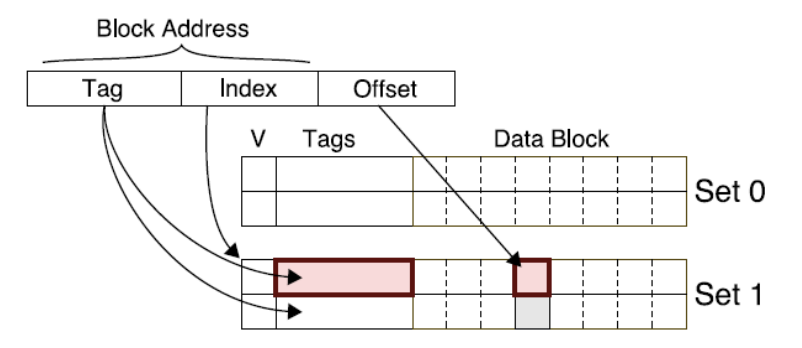
\includegraphics[width=0.5\textwidth]{2way-8-4line.png}
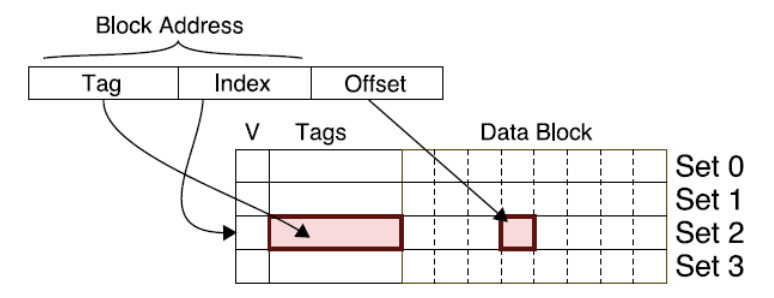
\includegraphics[width=0.5\textwidth]{direct-8-4line.png}

\subsection{Block Replacement}

We have no choice in a direct mapped cache, but in an associative cache, we can use random, LRU, FIFO (for highly associative caches), NMRU.

\subsection{Write Strategy}

For a cache hit, we can either do:
\begin{itemize}
\item \textbf{Write Through:} write both cache and memory, generally higher traffic but simpler to design
\item \textbf{Write Back:} write cache only, memory is written when evicted, dirty bit per block avoids unnecessary write backs, more complicated
\end{itemize}
For a cache miss, we can either do:
\begin{itemize}
\item \textbf{No Write Allocate:} only write to main memory
\item \textbf{Write Allocate:} fetch block into cache, then write
\end{itemize}
Usually we do either (1) write through and no write allocate or (2) write back and write allocate.

\subsection{Types of Cache Misses}

\begin{enumerate}
\item \textbf{Compulsory:} happens on first reference to block, can be somewhat resolved with prefetching
\item \textbf{Capacity:} happens because cache is too small to hold all data needed by program
\item \textbf{Conflict:} misses that occur because of collisions due to less than full associativity
\end{enumerate}

\subsection{Cache Optimizations}

\begin{enumerate}
\item Larger block size to reduce miss rate
\item Larger cache to reduce miss rate
\item Higher associativity to reduce miss rate
\item Multilevel cache to reduce miss penalty
\item Give priority to read misses over write misses to reduce miss penalty
\end{enumerate}

\subsection{Cache Size Equations}
$$ \text{Physical address size} = \text{Tag field size} + \text{Index field size} + \text{Offset field size} $$
$$ \text{Set associativity} = \frac{\text{Number of ways}}{\text{Set}} = \frac{\text{Number of blocks}}{\text{Number of sets}} $$
$$ 2^{\text{Index size}} = \frac{\text{Cache size}}{(\text{Block size}) \cdot (\text{Set associativity})} = \text{Number of sets} $$
$$ \text{Cache Memory Required} = (\text{Number of blocks}) \cdot \left( \underbrace{1}_\text{Valid bit} + (\text{Tag field size}) + (2^\text{Offset field size}) \cdot ( \text{Block size} ) \right) $$
Note: above there may also be another bit for LRU.

\subsection{Possible Questions}

\begin{enumerate}
\item Given a specification of a cache and its policies, as well as a sequence of memory access addresses, determine which accesses will produce cache hits and misses and also determine what kind of locality is in play (Spatial/Temporal/None). For the cache misses, indicate the type of cache miss (three C's). (Appeared in PS1 Q8, 2018 Midterm Q7)

\textit{Answer: simulate cache behavior---when switching between memory block accesses, call it temporal locality, and when accessing nearby addresses memory block call it spatial locality (miss = none)}

\item What are two common cache write strategies for cache [hits/misses] and what are the advantages and disadvantages of each?

\textit{Answer: see above}

\item Given a certain cache specification, which memory blocks can reside in each cache block? (Appeared in PS1 Q4)

\textit{Answer: use cache associativity to determine number of blocks/sets/ways and then use block placement strategy to determine where each memory block will go}

\item Name $n$ cache optimizations and whether they improve miss rate or miss penalty.

\textit{Answer: see cache optimizations above}

\item Draw a circuit diagram for an $n$-way set-associative cache with given block size and number of blocks. Show how address is split into fields and how multiplexing happens. Also give the total size of the cache and its fields. (Appeared in PS1 Q5, 2013 Midterm Q3, Coursera Midterm Q3, 2012 Final Q7)

\textit{Answer: use diagrams in block identification as reference but explicitly draw out tag/index checking and multiplexing---use cache size equations to determine cache size}
\end{enumerate}

\section{Interrupts/Exceptions}

\subsection{Interrupts}

An interrupt is an event that needs to be processed by another (system) program. The event is usually unexpected or rare from program’s point of view. The procedure is to go out to the interrupt handler and then continue afterwards.

\subsection{Asynchronous (external) interrupts}

When the processor decides to process the 
interrupt it stops the current program at instruction $I_i$, completing all the instructions up to $I_i-1$ (a precise interrupt). Then it saves the PC of instruction $I_i$ in a special register (EPC) and disables interrupts and transfers control before going to kernel mode

\begin{itemize}
\item Input/output device service request 
\item Timer expiration
\item Power disruptions, hardware failure
\end{itemize}

\subsection{Synchronous interrupts (exceptions/traps)}

In general, the instruction cannot be completed and 
needs to be restarted after the exception has been handled. This requires undoing the effect of one or more partially executed instructions or in the case of a system call trap, the instruction is considered to have been completed. We want to kill the oldest instruction.

\begin{itemize}
\item Undefined opcode, privileged instruction 
\item Arithmetic overflow, FPU exception 
\item Misaligned memory access  
\item Virtual memory exceptions: page faults, TLB misses, protection violations 
\item Software exceptions: system calls, e.g., jumps into kernel  
\end{itemize}

\subsection{Possible Questions}

\begin{enumerate}
\item Describe in the MIPS instruction set what state needs to be saved by the hardware interrupt mechanism. (Appeared in PS2 Q3a)

\textit{Answer: program counter (EPC), cause, and disabling of further interrupts (EXL=1)}

\item Describe in the MIPS instruction what happens on ERET? (Appeared in PS2 Q3b,c)

\textit{Answer: PC = EPC, old registers restored, enable interrupts (EXL=0)}

\item An instruction takes two synchronous exceptions $A$ and $B$.  What should the interrupt cause be loaded with?  What if that same instruction has an external interrupt pending? Explain. (Appeared in PS2 Q4, Coursera Midterm Q5)

\textit{Answer: the cause should be loaded with whichever exception would be caught further down in the pipeline, because this would correspond to an older instruction---if that same instruction has an external interrupt pending, we can take either, but usually we take the internal one to prevent external requests from hogging resources}

\item Name $n$ different causes for [a]synchronous interrupts?

\textit{Answer: see above}
\end{enumerate}

\section{Superscalars}

\subsection{Parallel Pipelines and Multiple Issue}
It is possible to have multiple pipelines that have different functions. In this way, we do not need the same number of cycles for every instruction type. Structural hazards are usually resolved in the decode stage. Multiple issue is when we try to execute more than one instruction at once. We may need to use swizzlers (instruction steering muxes) to make sure the instructions are routed to a pipeline that can handle them. We usually split the decode into two stages also---the decode and issue stages.

\subsection{Out-of-Order (OOO) Execution}
For naming classes of OOO processors, we use an I if in-order and an O if out-of-order. We can classify each OOO processor by its (1) frontend, (2) issue, (3) writeback, and (4) commit. We also abbreviate using numbers---for example, I2O2, means in-order frontend+issue, and out-of-order writeback+commit. \\
\\
The popular ones are:
\begin{itemize}
\item \textbf{I4:} scoreboard, fixed-length pipelines, no commit stage
\item \textbf{I2O2:} scoreboard
\item \textbf{I2OI:} scoreboard, reorder buffer, store buffer
\item \textbf{IO3:} scoreboard and issue queue
\item \textbf{IO2I:} scoreboard, issue queue, reorder buffer, store buffer
\end{itemize}

\subsection{Scoreboard}
This is an indexed register dependency tracker which denotes which functional unit is writing a register, whether or not the register is pending, and also which stages have an instruction that plans to write to the register.

\subsection{Reorder Buffer (ROB)}
For each physical register, we have state (empty, pending, finished), a speculative bit (for branches), a store bit, a valid bit and the physical register we are tracking with the entry. We also have a head and tail pointer that tracks which entries are in play. The reorder buffer makes sure that we commit in order---once the instruction at the head of the ROB is finished, it increments. On a branch, we squash all speculative instructions in ROB. Three possible designs with decreasing complexity based on when to squash speculative instructions and deallocate ROB entry: (1) as soon as branch resolves, (2) when branch commits, or (3) when speculative instructions reach commit. Our base design only allows one branch at a time---a second branch stalls in decode. We can add more bits to track multiple in-flight branches. 

\subsection{Register File}
\textbf{Architectural Register File (ARF):} committed state of the machine \\
\textbf{Physical Register File (PRF):} uncommitted state of the machine \\
\\
We must copy the contents of the ARF to the PRF on a branch mispredict to rollback after the branch has committed.

\subsection{Finished Store Buffer (FSB)}
This is a buffer that ensures that captures store data in a buffer before it is committed in case a load with the same address comes along before it completes. This is checked by load instructions before going to the cache.

\subsection{Issue Queue (IQ)}
This contains the operation, immediate value, speculative bit, destination+valid, src0+valid/pending, and src1+valid/pending.

$$ \text{Instruction Ready} = (!Vsrc0 \, || \, !Psrc0) \, \&\& \, (!Vsrc1 \, || \, !Psrc1) \, \&\& \, (\text{no structural hazards}) $$
For high performance, we can factor bypassing into the instruction ready equation.

\subsection{Register Renaming}

To fix WAW and WAR dependencies, we can do register renaming. Here, we map larger namespace of \textbf{physical registers} to a smaller namespace of \textbf{architectural registers}. In doing this, we modify our ROB to include the architectural register and the previous physical register. We also add a rename table and a free list to keep track of our mappings and which registers are free to be mapped.

\subsection{Rename Table (RT)}

Contains entries for each architectural register, and which physical register it maps to (as well as a pending bit). Requires:
$$ \text{Bits for RT} = N_{AR} * (1 + \log_2 N_{PR}) $$
We may also be allowed to exclude pending bit and/or register 0 from our calculations.

\subsection{Free List (FL)}

Contains indexed entries for each architectural register and one bit for whether or not it is free. Simple optimization on RT.

\subsection{Memory Disambiguation}

We need to make sure memory operations happen in a safe order:
\begin{enumerate}
\item \textbf{In-order memory queue:} makes sure that all loads/stores do not leave IQ until all previous loads/stores have completed
\item \textbf{Conservative OOO execution:} split execution of store into address calculation and data write, can execute load before store if addresses are different, stall if any previous store address is not known
\item \textbf{Address speculation:} we can guess that there is no problem, but if there is, we need to squash load and all following instructions, then restart; this can have a large penalty
\end{enumerate}

\subsection{Possible Questions}
\begin{enumerate}

\item Does each instruction need to take the same amount of cycles in a microcoded processor? Explain. (Appeared in 2018 Midterm Q1)

\textit{Answer: no, we can have asymmetric parallel pipes in a pipeline or we can have a multi-cycle processor which does the same thing}

\item Explain the conditions under which crossover would be needed in a pipeline. (Appeared in 2018 Midterm Q2)

\textit{Answer: in a dual-issue processor when we have asymmetric parallel pipes that can only execute certain kinds of instructions, we may need to route instructions to a pipe that can handle them}

\item Given [I4, I2O2, I2OI, IO3, IO2I] pipeline with certain features, show the pipeline diagram for the given code sequence executing. How many cycles does the code sequence take to complete? (Appeared in PS2 Q1, PS2 Q5, PS2 Q6, 2018 Midterm Q4, 2013 Midterm Q5a,c)

\textit{Answer: same as before but obey OOO properties of pipeline and remember issue/commit stages}

\item Given [I4, I2O2, I2OI, IO3, IO2I] pipeline with certain features, show the pipeline diagram for the given branch code sequence executing. How many instructions are squashed by the branch? (Appeared in PS2 Q2, Coursera Midterm Q6-17)

\textit{Answer: same as above; squash when possible then count all instructions below branch (including itself)}

\item What processor hardware structure provides $x$ feature? (Appeared in 2013 Midterm Q1, Coursera Midterm Q1)

\textit{Answer: see above}

\item Which data hazards is register renaming able to overcome? Will register renaming improve the performance of the given code sequence on processor with specified properties? (Appeared in Coursera Midterm 2, Coursera Midterm 14, Coursera Midterm 17)

\textit{Answer: WAW and WAR---find these dependencies and draw out pipeline diagram to see if stalling is necessary---if so, register renaming will help, else no}

\item Will an [I4, I2O2, I2OI, IO3, IO2I] pipeline with certain features have problems with precise interrupts? If so, give an example. (Appeared in 2013 Midterm Q5b)

\item Given [I4, I2O2, I2OI, IO3, IO2I] pipeline with certain features, show the state of the processor for $n$ cycles into the future? (Appeared in 2013 Midterm Q6)

\textit{Answer: simulate pipeline based on functionality of each component}

\item How do the hardware structures of a processor need to be modified when extending a scalar processor to a dual-issue superscalar processor? What parts of the Iron Law are affected? (Appeared in 2018 Midterm Q9, 2013 Midterm Q3)

\textit{Answer: register file needs twice as many read ports (4 read ports), register file needs twice as many write ports (2 write ports), fetch bandwidth needs to be doubled, decode logic needs to be duplicated, if full-bypassing is supported, cross-pipeline bypassing is needed, if pipelines are asymmetric, steering logic is needed---we get increased IPC at the possible cost of a lower clock rate}

\item Draw $x$ hardware structure from a superscalar processor with given properties. How many bits are required? (Appeared in 2018 Midterm Q8a,b)

\textit{Answer: see details of each structure above}

\item What are $n$ distinct ways of solving the memory disambiguation problem?

\textit{Answer: see above}

\item Suppose a processor takes an interrupt in an asymmetric pipe where there is an instruction in the shorter pipe. Under what circumstances will the instruction in the shorter pipe commit? Give a piece of example code. (Appeared in 2013 Midterm Q8a)

\textit{Answer: when an instruction in a longer pipe came before it. An example would be in a 4-stage MUL pipe if we do a MUL and then an ADD, we would need to commit in order to have precise exceptions.}

\item How could we have an empty pipe in an asymmetric parallel pipeline scenario? (Appeared in 2013 Midterm Q8b)

\textit{Answer: have multiple instructions that can only go down a particular pipe due to pipeline restrictions}
\end{enumerate}

\section{Very Long Instruction Word (VLIW)}

\subsection{Motivation}

If $W$ is the issue width, and $L$ is the lifetime ($\propto$ length of pipeline), each issued instruction must check against $W*L$ instructions. So we want to do the dependency checking in the compiler to reduce the complexity of the hardware---we put multiple ops into a bundle such that there are no RAW dependencies and each operation slot is for a fixed function. VLIWs may be a better way to represent control flow graphs (CFGs) rather than trying to parse them out in hardware.

\subsection{Scheduling Models}

\textbf{EQ Scheduling Model:} each operation takes exactly specified latency; interrupts cause problems, but can reuse registers quickly \\
\textbf{LEQ Scheduling Model:} each operation takes $\leq$ a specified latency; enables precise interrupts and increasing the processor speed means there are no problems

\subsection{Predication}

This is when we do:
$$ a = c \, ? \, d : e $$
The instructions to do this look like: \\
\texttt{movz rd, rs, rt \hspace{3cm} if (R[rt] == 0) then R[rd] $\leftarrow$ R[rs]} \\
\texttt{movn rd, rs, rt \hspace{3cm} if (R[rt] != 0) then R[rd] $\leftarrow$ R[rs]} \\
\\
There is also \texttt{slt} for ``set less than''. Predication does not help for long loop bodies, but helps for small ones. It turns control flow dependencies into data flow dependencies and can execute both sides at once on a VLIW---however it may require an extra read port on the register for writing same register. We also need to bypass predicates and need an RF for them. \\
\\
\textbf{Speculative execution} is when we move instructions across branches or move memory operations across branches. \textbf{Code motion} is valid reordering of code for better performance; for example, we can push loads up and stores down. \\
\\
Below are the complete steps for solving a \textbf{partial-predication} problem:
\begin{enumerate}
\item Identify the predication register. This is the register that is used for the conditional branch.
\item Identify the two code blocks.
\item Remove branches and jumps and rename conflicting variables between code blocks for the smaller block.
\item Add predication for one side---pick the smaller block to minimize running time. Do not worry about temporary variables, these do not matter.
\end{enumerate}

\subsection{Software Pipelining}
We need to do \textbf{loop unrolling} in order to access parallelism. The number of times to unroll the loop is called the \textbf{unroll factor} and we want this to be the latency of our longest instruction in the loop. \\
\\
We need to add a prolog to fill the pipe (with loads usually), and an epilog to clean up for iteration counts that are not multiples of the unrolling factor. We do the cleanup by adding a branch back to the epilog. Below are the complete steps for solving a software pipelining problem:
\begin{enumerate}
\item Determine unroll factor $u$ by examining code loop and finding instruction with longest latency.
\item Write out unrolled code in high-level language form for understanding.
\item Draw a table with rows being each VLIW and columns being the pipelines.
\item Every $u$ instructions should be a repetition in each pipe---repeat until the pipeline is full. Remember to increment the counter every $u$th instruction.
\item Loop section should be where pipeline is full. Remember to add the branch at the end of the loop in an available pipe.
\item The epilog should be the same length as the prolog and should phase out the instructions in the order they were originally, unless the iteration count is divisible by the unroll factor in which case no branches are needed.
\end{enumerate}
\textbf{Exam tip: do not bother writing out the full instructions for anything except inside the loop! Just write out the op names as this has minimal point value.}

\subsection{Trace Scheduling}

For trace scheduling, we pick a string of basic blocks, called a \textbf{trace} and form a \textbf{superblock} based on the most frequent branch paths. We can use profiling feedback or compiler heuristics to find common branch paths. We also need to add fix-up code to cope with branches escaping the trace.

\subsection{Problems with VLIW}

\begin{itemize}
\item \textbf{Object-code compatibility:} have to recompile all code for every machine, even within generation
\item \textbf{Object-code size:} instruction padding wastes instruction memory/cache, software pipelining replicates code
\item \textbf{Scheduling variable-latency memory operations}: caches and/or memory bank conflicts impose statically unpredictable variability
\item \textbf{Knowing branch probabilities:} profiling is significant extra step in build process
\item \textbf{Scheduling for statically unpredictable branches:} optimal schedule varies with branch path
\item \textbf{Precise interrupts can be challenging}: will fault in one portion of bundle fault whole bundle?
\end{itemize}

\subsection{Possible Questions}

\begin{enumerate}
\item What instruction set addition enables control flow to be turned into a data dependency? (Appeared in 2013 Midterm Q2)

\textit{Answer: predication}

\item Add partial-predication into the given code, minimizing running time using MOVZ and MOVN (conditional move instructions). Under what circumstances does it make sense to predicate? (Appeared in 2018 Midterm Q5, 2013 Midterm Q7, 2012 Final Q2d)

\textit{Answer: use partial-predication steps, then determine difference between average instruction count without predication versus instruction count with predication---take difference and multiply by two---this number is the branch predict penalty beyond which it makes sense to predicate (assuming a 50-50 unpredictable branch)}

\item Optimally schedule and bundle the given sequential code for a VLIW processor using the [EQ/LEQ] scheduling model. As a secondary constraint, minimize register usage. (Appeared in 2018 Midterm Q6, 2012 Final Q3)

\textit{Answer: use software pipelining steps}

\item List $n$ problems with classic VLIW.

\textit{Answer: see above}
\end{enumerate}

\section{Branch Prediction}

\subsection{Static Prediction}

\textbf{Always Predict Taken/Not Taken:} not taken is what we have been assuming, taken is difficult because we do not know the target until later \\
\textbf{Branch Delay Slot:} ISA semantics are changed so that the instruction(s) following a jump/branch is/are always executed \\
\textbf{Backwards Taken Forward Not Taken (BTFNT):} prediction based on static probabilities \\
\textbf{Extend ISA to Specify Prediction Statically:} we can add instructions like \texttt{BR.T} and \texttt{BR.NT} for this purpose

\subsection{Dynamic Prediction}

\textbf{One-bit saturating counter:} always predict the last outcome of the branch (temporal correlation in branch outcome), always mispredicts twice though at beginning and end \\
\textbf{Two-bit saturating counter:} have weak taken and weak not taken intermediate states that enable hysteresis, or could jump directly from strong to weak \\
\textbf{Branch history register (BHR):} records direction of last $N$ branches executed by processor (globally) \\
\textbf{Pattern history table (PHT):} BHR indexes this, recording what the past outcomes have been for specific pattern, driving FSM output logic \\
\textbf{Two-level branch predictor:} BHR indexes first PHT which indexes another PHT up to $2^{k-1}$ PHTs, then the branch address middle bits are used to select which PHTs output to use to drive FSM output logic---this approach can be generalized to have BHRs indexed by branch address middle bits so the branch history becomes local \\
\textbf{Tournament predictor:} a choice predictor based on branch address middle bits is used to outputs of a global predictor and a local predictor

\subsection{Branch Target Buffer (BTB)}

Uses branch middle bits to cache branch target from previous runs of instruction. This means we may not have to wait until the branch target is computed. We also keep track of the branch predictor's state from before. BTB is only updated for control instructions since all other instructions have \texttt{PC Next = PC + 4}.

\subsection{Possible Questions}

\begin{enumerate}

\item Briefly describe the purpose of the Branch Target Buffer (BTB). (Appeared in 2012 Final Q1)

\textit{Answer: The BTB allows the fetch stage of the pipeline to predict the address of the next instruction without having to decode the instruction. It is indexed by the current PC and outputs the next PC. Without the BTB, the pipeline would have to wait until the branch is decoded to determine the next PC. Otherwise the pipeline could just predict only fallthrough}

\item Given a prediction scheme and a piece of code, simulate the predictor and give its accuracy. (Appeared in 2012 Final Q2a,b,c)

\textit{Answer: simulate predictor as described above}

\end{enumerate}

\section{Advanced Cache Optimization}

\subsection{Pipelining Cache Writes and Write Buffers}

In the memory stage with pipelined cache writes, instead of writing back, we put data in a delayed cache write buffer. This helps memory bandwidth in the case where we write to a single address multiple times---we only need to writeback once for many writes---but it hurts the hit time. \textbf{Write buffers} are essentially the same thing, but exist on writeback lines from L1 to L2 cache; this helps the miss penalty.

\subsection{Multilevel Caches}

The miss rate equations are:
$$ \text{Local miss rate} = \frac{\text{Misses in cache}}{\text{Accesses to cache}} $$
$$ \text{Global miss rate} = \frac{\text{Misses in cache}}{\text{CPU memory accesses}} $$
$$ \text{Misses per instruction} = \frac{\text{Misses in cache}}{\text{Number of instructions}} $$

\begin{itemize}
\item Use a smaller L1 cache if there is also an L2 cache present
\begin{itemize}
\item Trade increased L1 miss rate for reduced L1 hit time and reduced L1 miss penalty
\item Reduce average access energy
\end{itemize}
\item Use simpler write-through L1 with on-chip L2
\begin{itemize}
\item Write-back L2 cache absorbs write traffic, doesn’t go off-chip 
\item At most one L1 miss request per L1 access (no dirty victim write-back) simplifies pipeline control 
\item Simplifies coherence issues 
\item Simplifies error recovery in L1 (can use just parity bits in L1 and reload from L2 when parity error detected on L1 read)
\end{itemize}
\end{itemize}
Multilevel caches improve miss rate and miss penalty.

\subsection{Multilevel Inclusion Policy}

\textbf{Inclusive multilevel cache:}
\begin{itemize}
\item Inner cache holds copies of data in outer cache 
\item External coherence snoop access need only check outer cache
\end{itemize}
\textbf{Exclusive multilevel caches:}
\begin{itemize}
\item Inner cache may hold data not in outer cache 
\item Swap lines between inner/outer caches on miss
\item Stores more data
\end{itemize}

\subsection{Victim Caches}

A victim cache is a small fully associative cache for recently evicted lines. If something keeps getting evicted, we make it quick to put it back in the cache. A victim cache is usually write-through, which keeps it clean. It is designed to reduce conflict miss rate and miss penalty.

\subsection{Prefetching}

This is where we speculate on future instruction/data accesses and fetch them into cache---this can be done in hardware/software/both. It is important to produce mostly hits, not be too early/late, and not pollute the cache/bandwidth. Prefetching reduces the miss rate and the miss penalty.

\subsection{Multiporting and Banking}

Multiporting and banking are techniques designed to increase cache bandwidth. One challenge with multiporting is deciding what happens if we have two stores or a load and a store to the same line. Multiporting is also costly---it can increase area by a lot and hit time by some too. A solution is \textbf{banked caching}, where address space is partitioned into multiple \textbf{banks}. This enables higher throughput, but there can be bank conflicts and extra wiring is required.

\subsection{Compiler Optimizations}

\begin{enumerate}
\item \textbf{Loop interchange:} when we have a 2D/higher-dimensional array access, we can flip the for loop order to improve spatial locality
\item \textbf{Loop fusion:} if we are iterating over two independent arrays of the same size in two separate loops, we can combine the loops into one, improving temporal locality
\item \textbf{Matrix multiply with cache tiling/blocking:} improve spatial locality by doing multiplication in blocks rather than over the entire matrix at once
\end{enumerate}
Overall, these optimizations reduce the miss rate.

\subsection{Non-Blocking Caches}

We can allow more cache accesses even after a miss occurs---both hit-under-miss and miss-under-miss (concurrent misses) are possible. The challenges are maintaining order when multiple misses happen that might return out of order, or we load/store to an already pending miss address. A \textbf{Miss Status Handling Register (MSHR)}/\textbf{Miss Address File (MAF)} and a load/store entry table are needed to keep track of the addresses; on a cache miss, the MSHR is checked for a matching address---if found, a new load/store entry is allocated pointing to MSHR, else both a new entry and a load/store entry are allocated. When MSHR is full, the processor stalls or prevents new loads/stores. When data is returned from memory, it can forward it to the processor and write the cache line. Once the cache line is written, the MSHR entry can be deallocated. With an in-order pipeline, a scoreboard is needed. Overall, non-blocking caches improve miss penalty and bandwidth.

\subsection{Critical Word First and Early Restart}

We want to pull the block we need in first, and the rest of the cache line can come later. With early restart, data returns from memory in order and the processor restarts when the needed word is returned. This reduces the miss penalty.

\subsection{Possible Questions}

\begin{enumerate}

\item Explain what a write buffer does and what it does to improve performance.

\textit{Answer: see above}

\item Given a profile with numbers for misses in cache, accesses to cache, CPU memory accesses, and number of instructions, give local/global miss rate and misses per instruction.

\textit{Answer: see multilevel cache formulas}

\item Explain the difference between inclusive and exclusive multilevel caches.

\textit{Answer: see above}

\item What is the problem with multiporting? What advantages does banking have over it?

\textit{Answer: see above}

\item Name $n$ compiler optimizations and explain how they improve performance.

\textit{Answer: see above}

\item Explain how a non-blocking cache works.

\textit{Answer: see above}

\item Fill in the chart for which factors (bandwidth, miss/hit rate, miss/hit time) are affected by different cache optimizations.

\textit{Answer: see above}

\item Which cache has better performance and by how much given hit/miss rates and hit/miss times? (Appeared in HW4 Q1)

\textit{Answer: use weighted sum formula}

\item If we use critical word first and early restart with given page size, cache size, latencies, how many cycles with/without critical word first? (Appeared in HW4 Q2a)

\textit{Answer: with critical word first, the only cost is the initial overhead---for non-critical word first, take into account per-block cost. If data can be directly bypassed to the read port of the L2 cache, we can ignore the overhead for writing cycles to the L2 cache}

\item Does critical word first and early restart help more for L1 or L2 caches? Which factors determine relative importance? (Appeared in HW4 Q2b)

\textit{Answer: they help with L1 caches more, since the L1 cache is accessed more frequently than the L2 cache. However, if we are going out to the L2 cache a lot i.e. lots of L1 cache misses, then adding CWF+ER to the L2 cache will help more since the L2 cache is slower. So the two factors are (1) frequency of cache access, and (2) speed of cache}

\end{enumerate}

\section{Address Translation and Protection}

\subsection{Components of Memory Management}

\textbf{Translation:} mapping of virtual address to physical address \\
\textbf{Protection:} permission to access word in memory \\ 
\textbf{Virtual Memory:} transparent extension of memory space using slower disk storage 

\subsection{Dynamic Address Translation}

This enables programs to operate independent of their location in memory. The simplest form is \textbf{base-and-bound translation}, which adds base+bound registers and checks whether an address is outside of these---if so, a bounds violation is raised. This can also enable separate areas for program and data, which is advantageous because it prevents a program from overwriting itself. The problem with contiguous memory systems is fragmentation---it becomes difficult to reuse memory for new programs after a while.

\subsection{Paged Memory Systems}

We provide different \textbf{page tables (PTs)} for different processes, which gives the illusion of a private address space that maps to non-contiguous physical memory. A processor-generated address is interpreted as a pair $<$page number, offset$>$---the offset is never translated. Space required by a page table is proportional to the address space, number of users, inverse to size of each page. PTs are usually kept in main memory. Linear PTs have a page table base register that is set whenever the active user process changes and contain in their entries (PTEs):
\begin{itemize}
\item A bit to indicate if a page exists 
\item PPN (physical page number) for a memory-resident page 
\item DPN (disk page number) for a page on the disk 
\item Status bits for protection and usage
\end{itemize}
Applications should never be allowed to touch page tables (either their own or others')---this should be handled by the OS.

\subsection{Hierarchical Page Tables}
Hierarchical page tables can prevent memory blowup by dividing index space into multiple levels that require less space in memory. For example a single-level page table with 24-bit VPN requires $2^{24}$ entries, but a two-level page table could use $2^{12}$ entries for each level, so $2^{13}$ total entries. Protection checks are also easy to build into page tables. Status bits are only needed for the lowest-level pages (leaves). \\
\\
Length of fields for page table:
$$ \text{Offset field size} = \log_2(\text{PPN size}) $$
$$ \text{VPN size} = \text{Virtual address length} - \text{Offset field size} - \text{Overhead (if any)} $$
$$ \text{PTE size} = 2^{\lceil \log_2(\text{VPN size} + \text{Status bit overhead size}) \rceil} $$
$$ \frac{\text{PTEs}}{\text{Page}} = \frac{\text{Page size}}{\text{PTE size}} $$
$$ \text{Number of page table levels} = \left\lfloor \frac{\text{PTEs}}{\text{Page}} / (\text{VPN size}) \right\rfloor $$
$$ \text{Maximum reach} = 2^{\text{VPN size}} $$
$$ \text{Minimum page table overhead} = \text{Number of page table levels} \cdot \text{Page size} $$

\subsection{Translation Lookaside Buffers (TLBs)}
These are translation caches, typically 16-128 entries and fully associative. Each entry maps a large page and sometimes larger systems can have multi-level TLBs to cache translations at each level. Usually replacement is done randomly (via clock) or via FIFO. \\
\\
The \textbf{TLB Reach} is the size of the largest virtual address space that can be simultaneously mapped by the TLB and is given by the formula:
$$ \text{TLB Reach} = \text{Number of TLB entries} \cdot \frac{\text{Number of pages}}{\text{TLB entry}} \cdot \text{Max page size} $$
TLBs can be extended with Address Space Identifier (ASID) that allows TLB entries from multiple processes to be in the TLB at the same time, with a global bit to match on all ASIDs. Also variable page sizes and a kernel/user mode bit can be added. \\
\\
TLBs can be physically indexed/physically tagged, virtually indexed/virtually tagged, virtually indexed/physically tagged, both indexed/physically tagged, but not physically indexed/virtually tagged.

\subsection{Address Translation Flowchart}

\begin{center}
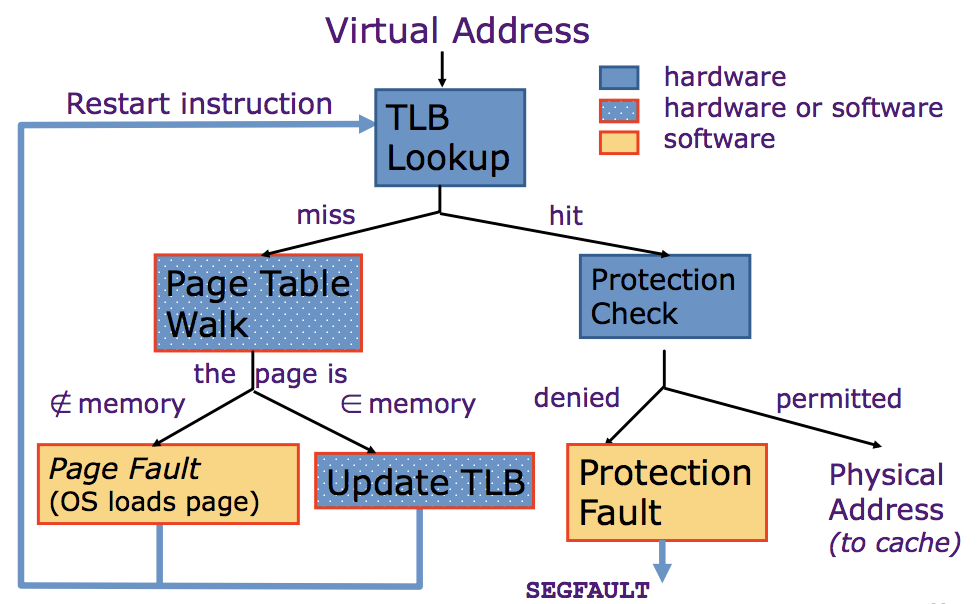
\includegraphics[width=0.75\textwidth]{addr-trans-flowchart}
\end{center}

\subsection{Demand Paging}
This uses a swapping store with lazy memory allocation to provide the ability to run programs larger than the primary memory. This also hides differences in machine configurations. The price is that address translation must be done on each memory reference.

\subsection{Possible Questions}

\begin{enumerate}
\item What is the reach of a TLB with $n$ entries and valid page sizes $p_1, p_2 ... p_n$? (Appeared in PS4 Q3)

\textit{Answer: $n \cdot \max(p_i)$}

\item Given virtual/physical address sizes, design a multi-level page table where the different levels fit within page of certain size. How many page table levels are needed and what is the minimum page table overhead if we store page tables in pages? What is the maximum reach of our paging system? (Appeared in PS4 Q4)

\textit{Answer: use hierarchical page table equations}

\item What are the possible reasons for a TLB miss in [software/hardware]-managed MMU? Does this always result in a bus-error/segfault? (Appeared in PS4 Q5)

\textit{Answer: possible reasons are (1) address is cached but was kicked out of the TLB, in which case it needs to be put back in TLB, (2) address is not cached, in which case we go out to main memory to get it via PT traversal. For hardware managed, we also have: (3) address is on not cached, and is on disk, in which case a page fault would happen and OS would take control, (4) none of the above, in which case there is a segfault}
\end{enumerate}

\section{Vector, SIMD, GPUs}

\subsection{SIMD/Multimedia Extensions}
We can use 64-bit registers as multiple $2^n$-bit registers where $n < 6$. Vector processors usually use deep pipelines and have no need for FU-internal bypassing since each vector element is independent. But we want to bypass between functional units to perform \textbf{vector chaining}, where there are dependencies between instructions. Vector chaining removes the need for a delay between iterations of a loop. If we add more RF ports and have a bypass network, we can even overlap two loop iterations almost entirely. CUDA uses \textbf{strip-mining} to create thread blocks, where loops are broken into pieces that fit in registers.

\subsection{Advantages of Vector Instruction Sets}
They are compact, scalable, and expressive (tell hardware that N operations are independent, use the same functional unit, access disjoint registers, access registers in the same pattern, access a contiguous block of memory, access memory in a known pattern). Vectorization is a massive compile-time reordering of operation sequencing. Full vector support adds better support for misaligned memory accesses.

\subsection{Vector Mask}

This is the vector version of predicate registers. This is how we can perform different operations on different pieces of a vector.

\subsection{Scatter-Gather}

\textbf{Scatter:} index with indexed array for store \\
\textbf{Gather:} index with indexed array for load

\subsection{GPUs/GPGPUs}

\textbf{Single Instruction, Multiple Data/Thread (SIMD/SIMT)} uses individual scalar instruction streams for each thread grouped together. There are many parallel cores, each with SIMD processor but no scalar processor---the CPU is the controller and the GPU carries out the work.

\subsection{Steps for Vector Pipelining Problems}

For a single-lane architecture with one write port and two read ports:
\begin{enumerate}
\item Write assumption that vector and scalar pipelines are decoupled, and we will only be focusing on the vector ones.
\item Identify vector operations in code given.
\item Find all data hazards.
\item Write out first line of first vector operation (as if it were a scalar). Remember that there should be a ``vector issue'' stage \textbf{R} after the decode stage.
\item For the next $n-1$ lines (where $n$ is the size of the vector being operated on), take everything from R until W and duplicate with shift of 1 for each line. Do not include anything before the R stage.
\item For the next instructions, do the same, but stall in each stage to ensure that there are no structural hazards. Ensure that data hazards are accounted for i.e. an instruction only begins when its operands are valuable. If a shorter instruction comes after a longer instruction, we will need to stall more than usual to make sure there is no structural hazard in the writeback stage.
\end{enumerate}

For a two-lane architecture with one write port and two read ports \textit{per lane}:
\begin{enumerate}
\item Write assumption that vector and scalar pipelines are decoupled, and we will only be focusing on the vector ones.
\item Identify vector operations in code given.
\item Find all data hazards.
\item Write out first line of first vector operation (as if it were a scalar). Remember that there should be a ``vector register read'' stage \textbf{R} after the decode stage.
\item For the next $(n-1)/2$ lines (where $n$ is the size of the vector being operated on), take everything from R until W and duplicate with shift of 1 for each line. Do not include anything before the R stage.
\item Copy the previous $n/2$ lines from the R stage after (without shifting) for the second lane.
\item For the next instructions, do the same, but stall in each stage to ensure that there are no structural hazards for the F and D stages only. Ensure that data hazards are accounted for i.e. an instruction only begins when its operands are valuable. We can have multiple instructions in R and W stages.
\end{enumerate}

\subsection{Possible Questions}

\begin{enumerate}

\item Do GPUs have vector length registers? Describe how they handle the case where two elements in a vector of data need different processing. (Appeared in PS4 Q8)

\textit{Answer: GPUs do not have vector length registers---instead they pack operations into SIMD style instructions, and if two elements need different processing, a vector mask is used to perform the operations in a predicated fashion}

\item Write out the vector pipeline diagram for a given segment of code running on a specified vector architecture with one or two lanes. (Appeared in PS4 Q6, PS4 Q7, 2012 Final Q4)

\textit{Answer: see steps for vector pipelining problems}

\item What are $n$ advantages of vector instruction sets?

\textit{Answer: see above}

\item What problem does vector stripmining solve? How is the Vector Length Register (VLR) involved with stripmining? (Appeared in 2012 Final Q5)

\textit{Answer: it allows loops larger than the VLR to execute; the VLR is set to maximum for most iterations and set to the remainder at the beginning/end}

\end{enumerate}

\section{Multithreading}

\subsection{Motivation}

Difficult to continue to extract instruction-level parallelism (ILP) or data level parallelism (DLP) for a single sequential thread of control. Instead, we can use thread level parallelism (TLP) where we specify independent sequential jobs. This can improve utilization of a single processor.

\subsection{Fine-Grain Multithreading}

We can remove data hazards in the pipeline by interleaving different independent threads. To modify the pipeline for this, we have 4 PCs and a rotating thread select which chooses which instruction goes next. This appears to software (including the OS) as multiple slower CPUs. \\
\\
The costs are that each thread requires its own user state and system state and there are other overheads from TLB/caches which need to be duplicated or have higher rates of conflict/capacity misses. \\
\\
For thread scheduling policies, we can use a fixed interleave or software/hardware-controlled interleave.

\subsection{Coarse-Grain Multithreading}

In coarse-grain multithreading, we swap threads on cache  misses to hide their latency. This is nice since some architectures do not have many low-latency bubbles.

\subsection{Simultaneous Multithreading (SMT)}

In an OOO superscalar, we can allow instructions from multiple threads to enter execution on the same clock cycle, giving better utilization of machine resources. We have an issue width and we interleave multiple threads to multiple issue slots with no restrictions. This prevents execution units from idling in an OOO superscalar. \\
\\
If we only do cycle-by-cycle interleaving i.e. vertical multithreading, we can remove some vertical waste but we still have some horizontal waste. \textbf{Chip multiprocessing}, where we split the chip horizontally has the opposite problem---we remove some horizontal waste but we still have some vertical waste.

\subsection{Multithreaded Categories}

\begin{center}
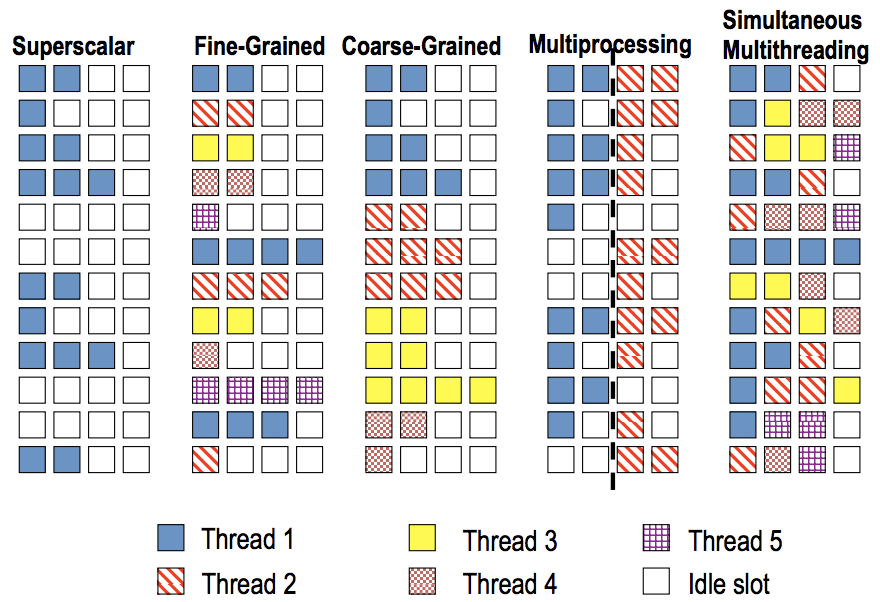
\includegraphics[width=0.75\textwidth]{multithreading}
\end{center}

\subsection{Possible Questions}

\begin{enumerate}
\item Given a piece of code, number of threads, description of L1 cache hits/misses, and specifications for three processors which have fine-grained, coarse-grained, and simultaneous multithreading, determine how many cycles each processor will take to execute. (Appeared in PS5 Q1)

\textit{Answer: use specifications and simulate execution---remember that all data+control+structural dependencies must be obeyed---also state all your assumptions and do not worry about cooldown, there will be minimal points for that}

\end{enumerate}

\section{Parallel Programming and Small Multiprocessors}

\subsection{Synchronization Models}

\textbf{Producer-Consumer:} In this synchronization scheme, a consumer process must wait until the producer process has produced data \\
\textbf{Mutual Exclusion:} In this synchronization scheme, only one process uses a resources at a given time

\subsection{Sequential Consistency}

This is an arbitrary order-preserving interleaving of memory references of sequential programs. SC basically adds dependencies between every instruction and the previous one.

\subsection{Semaphores}

A semaphore determines the maximum number of processes that can access a resource simultaneously. $P(s)$ decreases $s$ by 1 if $s > 0$, else the process waits, and $V(s)$ increases $s$ by 1 after a process is finished using the resource. So before a critical section, we want to run $P(s)$ and afterwards, we want to run $V(s)$. Semaphores can be implemented at the ISA level with:

\begin{enumerate}
\item \textbf{Test\&Set:} this writes 1 to a memory location if the data there is 0
\item \textbf{Fetch\&Add:} this adds a register value to a memory location
\item \textbf{Swap:} this swaps a register value and data a memory location
\item \textbf{Compare\&Swap:} this swaps a register value and data a memory location depending on whether it is equal to the value of another register
\item \textbf{Load-link/Store-conditional:} special registers hold reservation flag and address, returns status as success/failure
\end{enumerate}

\subsection{Relaxed Memory Models}

Memory fences can also be used to sequentialize memory accesses, but these are expensive. \\
\textbf{Total Store Order:} LL, LS, SS, enforce SL with fence \\
\textbf{Partial Store Order:} LL, LSm enforce SL, SS with fences \\
\textbf{Weak Ordering:} enforce LL, LS, SL, SS with fences

\subsection{Dekker's Algorithm}

This is an algorithm that ensures mutual exclusion with two processes (was extended to $n$ processes by Dijkstra but is complicated):
\begin{center}
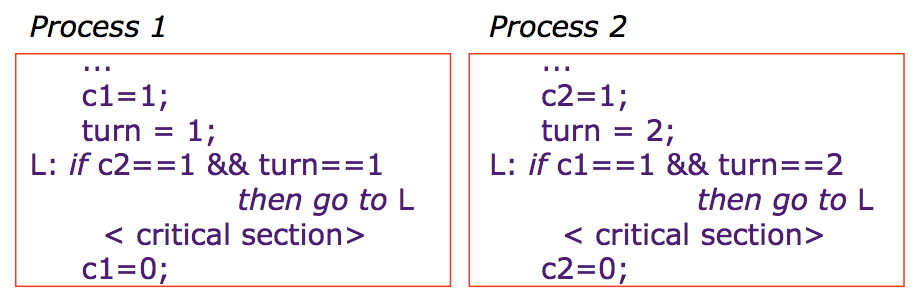
\includegraphics[width=0.75\textwidth]{dekker}
\end{center}

\subsection{Lamport's Bakery Algorithm}

\begin{enumerate}
\item Set \texttt{choosing} for $i$th process to 1.
\item Take the next ticket by looking at everyone's ticket and adding one to the highest one.
\item We are done choosing now, so set \texttt{choosing} back to 0.
\item Now iterate over all processes: for each, let process finish choosing, then see if we are the lowest ticket number (using process number as tiebreaker). If so, enter critical section, if not, spin until the resource is released.
\item To release resource, set ticket number to 0.
\end{enumerate}

\subsection{Symmetric Multiprocessors (SMPs)}

In this model, all memory is equally far away from all processors and any processor can do any I/O---we also have a pipelined memory bus. The question is how to do memory coherence in SMPs with write-back/write-through. Write-back results in main memory and other cache having stale values and write-through results in other cache having stale values. Stale values lead to sequential inconsistency, because one processor could be working with old data. For this reason we need \textbf{cache coherence}.

\subsection{Cache Coherence vs. Memory Consistency}

A cache coherence protocol ensures that all writes by one processor are eventually visible to other processors, for one memory address i.e. updates are not lost, while a memory consistency model gives the rules on when a write by one processor can be observed by a read on another, across different addresses i.e. what values can be seen by a load. Together, sequential consistency can be implemented.

\subsection{Snoopy Cache Protocol}

In a snoopy cache, there is a bus on which all processors shout write updates/write invalidates via a broadcast mechanism. Write update means updates are shouted across bus and everyone has to update. Write invalidate means invalidate is shouted across bus and if someone wants to read, they have to ask for the data. Snooping uses a lot of bandwidth and arbitrating the bus atomically becomes a challenge.

\subsection{MSI Protocol}
M is for modified exclusive, I is invalid, S is shared. Each processor has two bits for every cache line.
\begin{center}
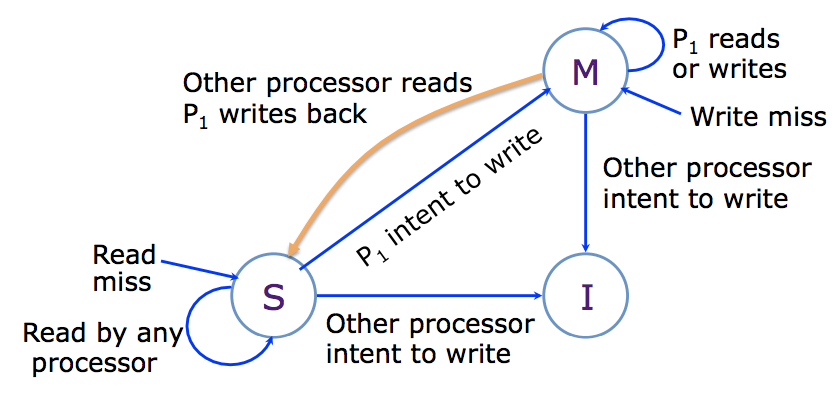
\includegraphics[width=0.75\textwidth]{msi}
\end{center}

\subsection{MESI Protocol}
M is for modified exclusive, E is for exclusive unmodified, I is invalid, S is shared. Each processor has two bits for every cache line, which are now fully utilized. This increases performance for private data with the exclusive state, which exists when a cache line is marked as not shared.
\begin{center}
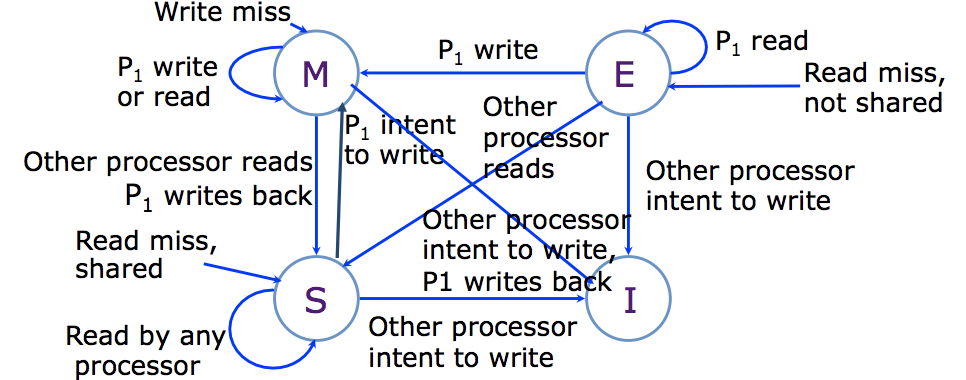
\includegraphics[width=0.75\textwidth]{mesi}
\end{center}

\subsection{MOESI Protocol}
M is for modified exclusive, O is for owned, E is for exclusive unmodified, I is invalid, S is shared. Each processor has two bits for every cache line. This is the same as MESI but we have extra information when we own the cache line.
\begin{center}
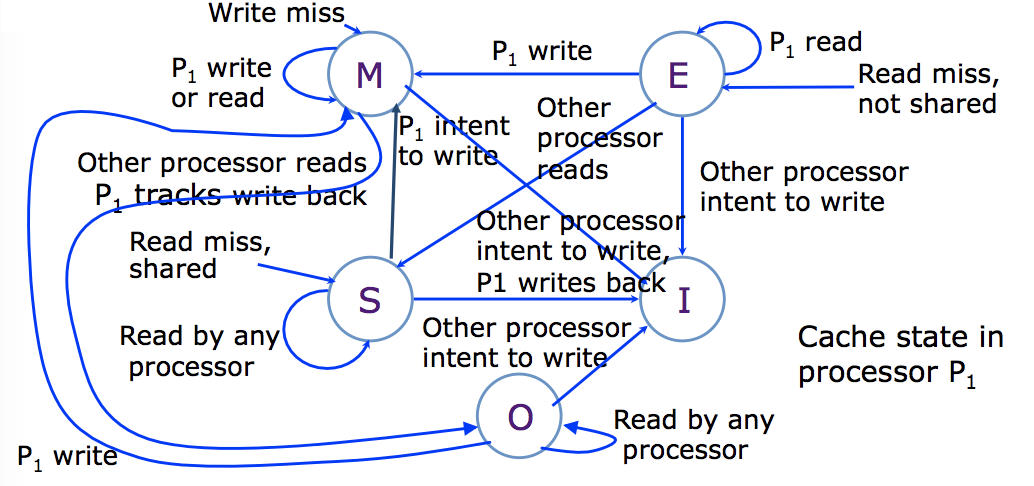
\includegraphics[width=0.75\textwidth]{moesi}
\end{center}

\subsection{MESIF Protocol}
M is for modified exclusive, E is for exclusive unmodified, I is invalid, S/F is shared/forward. Each processor has two bits for every cache line. Same as MESI but uses forwarding instead of invalidate.
\begin{center}
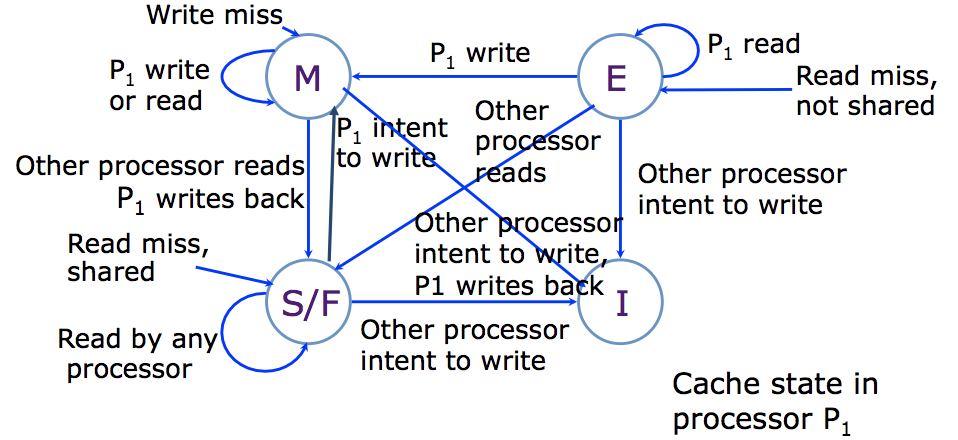
\includegraphics[width=0.75\textwidth]{mesif}
\end{center}

\subsection{False sharing}

This is when two processors try to write different words in the same block exclusively. The processors will then behave as if they are contending for a shared resource when really there is no need to be sharing at all.

\subsection{Possible Questions}

\begin{enumerate}

\item Write a code sequence showing false sharing. Assume that the code is running on a shared memory multiprocessor system with caches and denote what code executes on each processor and any assumptions about cache block size. (Appeared in 2012 Final Q8)

\textit{Answer: make the two processors write to two different places in the same block by making the offsets smaller than the block size at the same memory address}

\item Implement compare and exchange with test and set. (Appeared in PS5 Q2)

\textit{Answer: express memory as a pointer to a struct containing the data and the lock, then wait until test and set on the lock returns. Now we have the lock, so we can compare the data and then exchange the values of memory and the swap pointer if the compare value is equal, else do nothing. Release the lock by setting it to 0 after done. Return the status (whether the exchange occurred) in either case.}

\item For given sequences of code running on $n$ threads with some shared variables, what are legitimate final results for the shared variables under the sequential consistency model? (Appeared in PS5 Q3, 2012 Final Q9)

\textit{Answer: for each load and store, write out pseudo-code for what is happening, then find the code execution paths that could lead to each result and make sure both threads have to be executing in order i.e. if we had to order the operations with arrows, there would be no crossing arrows between threads}

\item Name $n$ atomic operations that are implemented in ISAs.

\textit{Answer: see above}

\item Multithread/add semaphores to a given piece of code with some shared memory like a counter or a frequency array. (Appeared in PS5 Q4, 2012 Final Q10)

\textit{Answer: make semaphores for each shared variable; initialize threads/locks, wrap usage of shared variables in \texttt{P()}s and \texttt{V()}s}

\item Write out pseudo-code for Dekker's/Lamport's bakery algorithm.

\textit{Answer: see above}

\item Show for each cache line and cache what state it is on every cycle for a sequence of loads/stores happening on $n$ processors over $T$ cycles assuming specified cache properties. Assume that [MSI/MESI/MESIF/MOESI] is used for caches. (Appeared in PS5 Q5, 2012 Final Q6)

\textit{Answer: simulate protocols as described above, watching out for cache line aliasing}

\item Write the state diagram for [MSI/MESI/MESIF/MOESI]. Extend this to work for directory coherence. (Appeared in PS5 Q10)

\textit{Answer: draw state machines as above, but add in what directory would do with stuff}

\end{enumerate}

\section{Interconnection Networks}

\subsection{Message Passing}

In message passing schemes, all memory is private, and explicit send/receives are used to communicate. This is easy for producer-consumer, but we need to know the destination on generation of data for sending. We can do messaging over shared memory and also shared memory over messaging.

\subsection{Message Anatomy}

A flit is a flow control digit (the basic unit of flow control), and a phit is a physical transfer digit (the basic unit of data transferred in one clock). We include the source, destination, length of message in the header and send this as a packet, which is a component of a message.

\subsection{Switching}
\textbf{Circuit Switched:} reserve the line as in a bus \\
\textbf{Store and Forward:} pass on each cycle\\
\textbf{Cut-through/Wormhole:} pass on in a pipelined fashion (not necessarily full message)

\subsection{Topology}

$k$-ary $n$-cubes are $n$-dimensional cubes with $k$ nodes along each dimension. $k$-ary $n$-tori are $k$-ary $n$-cubes with the ends connected. Crossbar networks are fully-connected networks. The above are all direct networks. Indirect networks include omega networks and fat trees in which the routers are not directly associated with a node. An omega network has depth $d$ and unidirectionally connects two nodes at every level to ensure that all nodes can route messages to each other in at least one way. Fat trees are bidirectional trees in which the router bandwidth is doubled at each level.

\begin{center}
\begin{tabular}{ c || c | c | c }
 \textbf{Topology} & \textbf{Diameter} & \textbf{Bisection Bandwidth} & \textbf{Router Degree} \\ 
 \hline \hline
 $k$-ary $n$-cube & $n(k-1)$ & $k^{n-1}$ & $2n + 1$ \\
 $k$-ary $n$-torus & $\sim n(k-1)/2$ & $\sim nk$ & $2n + 1$ \\
 crossbar & 1 & $N^2/2$ & $N$ \\
 omega network & $d+1$ & $N/2$ & 2 \\
 fat tree & $N$ & $2\log_2(N)$ & 3 \\
\end{tabular}
\end{center}
We typically do not want to pack greater than $N+1$ dimensions in $N$ space.

\subsection{Network Performance}

\textbf{Bandwidth:} the rate of data transmission over the network in a given time \\
\textbf{Latency:} the time taken for a message to be sent from sender to receiver \\
\\
Bandwidth can affect latency and vice versa---we can trade off bandwidth and latency. Bandwidth affects phit size which affects number of phits to send a message. \\
\\
$H_C$ is the hop count, $t_C$ is the channel latency (in cycles), $t_R$ is the router latency (in cycles), $T_{head}$ is the latency of the header packet (in cycles), $\text{Latency}_{ser}$ is the latency of serializing the message (in cycles)---below are equations for computing latency in a wormhole routing scheme:
$$ T_{head} = H_C \cdot (t_C + t_R) + t_R $$
$$ \text{Latency}_{ser} = L/b $$
$$ T = T_{head} + L/b $$
For a store and forward, we use the same scheme but the entire message must arrive before moving forward.

\subsection{Routing and Flow Control}

Routing can either be oblivious (deterministic/non-deterministic) or adaptive (the routing path depends on the state of the network). Flow control can either be local or end-to-end (planned over a long distance). We want to try to avoid deadlock or be able to recover from it with buffering. Credit-based flow control is where we increment a counter on receiving a credit, decrement it on sending a packet, and only send when we have available credits.

\subsection{Possible Questions}

\begin{enumerate}

\item Calculate the [diameter/bisection bandwidth/router degree] of a given topology under certain parameters. (Appeared in PS5 Q6)

\textit{Answer: use topology properties from above}

\item How large of a credit counter is needed to provide full bandwidth on a link where the link has $n$ cycles of latency in the path? What is the bandwidth as a fraction of the maximum if we decrease the credit size to $m$ smaller than the needed number? (Appeared in PS5 Q7)

\textit{Answer: $n + 1$ and $\frac{n+1-m}{n+1}$ respectively}

\item Given a topology with link/router/serialization delays and link/flit/phit/message sizes, how many cycles does it take to send a message from point $A$ to point $B$. (Appeared in PS5 Q8, 2012 Final Q11)

\textit{Answer: use equations for latency above}

\end{enumerate}

\section{Directory Cache Coherence}

\subsection{Motivation}

Snoopy protocols require every cache miss to be broadcast which requires a lot of bandwidth and a lot of snooping bandwidth. Directory protocols keep track of all caches holding a memory block and use point-to-point messaging to maintain coherence.

\subsection{Non-Uniform Memory Access (NUMA)}

Latency to access memory is different depending on node accessing it and address being accessed. We have an address to home directory. If we let the high-order bits determine home directory and the low-order bits determine index+offset, the OS has placement control---the problem is that homes can become hotspots for traffic. If we let the low-order bits determine home directory, the OS has little control over placement, but we get good load balancing for free.

\subsection{Full-Map Directory}

For each cache line, the directory contains the state that the directory believes cache line is in (shared, uncached, exclusive, (pending)) and the sharers/owner (depending on state). Basically it just keeps track of who cares about each cache line's data. Directories also are used as an ordering point---whichever message arrives first is taken, and other messages are given a NACK. But a forward progress guarantee is needed---after a node acquires a line, we need to commit at least one memory operation before transitioning, invalidating line.

\subsection{ESU Protocol}

This is the same as MSI but extended for directory cache coherence.
\begin{center}
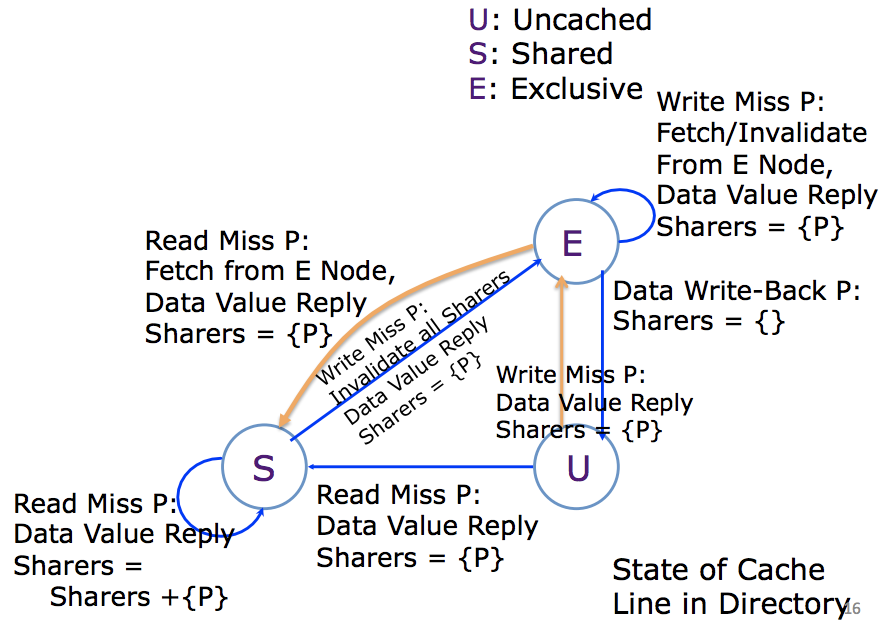
\includegraphics[width=0.75\textwidth]{esu}
\end{center}

\subsection{Possible Questions}

\begin{enumerate}

\item Show for each cache line, cache, and director controller what state it is on every load/store for a sequence of loads/stores happening on $n$ processors over $T$ cycles assuming specified cache properties. Assume that [MSI/MESI/MESIF/MOESI] is used for caches and ESU is used at the directory. (Appeared in PS5 Q9)

\textit{Answer: simulate protocols as described above}

\end{enumerate}

\end{document}
